\documentclass[
]{jss}

%% recommended packages
\usepackage{orcidlink,thumbpdf,lmodern}

\usepackage[utf8]{inputenc}

\author{
Boyi Guo\\University of Alabama at Birmingham \And Nengjun
Yi\\University of Alabama at Birmingham
}
\title{The R Package \pkg{BHAM}: Fast and Scalable Bayeisan Hierarchical
Additive Model for High-dimensional Data}

\Plainauthor{Boyi Guo, Nengjun Yi}
\Plaintitle{The R Package BHAM: Fast and Scalable Bayeisan Hierarchical
Additive Model for High-dimensional Data}
\Shorttitle{\pkg{BHAM}: Bayeisan Hierarchical Additive Model}


\Abstract{
\textbackslash pkg\{BHAM\} is a freely avaible R pakcage that implments
Bayesian hierarchical additive models for high-dimensional clinical and
genomic data. The package includes functions that generlized additive
model, and Cox additive model with the spike-and-slab LASSO prior. These
functions implements scalable and stable algorithms to estimate
parameters. \textbackslash pkg\{BHAM\} also provides utility functions
to construct additive models in high dimensional settings, select
optimal models, summarize bi-level variable selection results, and
visualize nonlinear effects. The package can facilitate flexible
modeling of large-scale molecular data, i.e.~detecting succeptable
variables and inforing disease diagnostic and prognostic. In this
article, we describe the models, algorithms and related features
implemented in \textbackslash pkg\{BHAM\}. The package is freely
avaiable via the public GitHub repository
\url{https://github.com/boyiguo1/BHAM}.
}

\Keywords{additive model, spike-and-slab LASSO, scalable}
\Plainkeywords{additive model, spike-and-slab LASSO, scalable}

%% publication information
%% \Volume{50}
%% \Issue{9}
%% \Month{June}
%% \Year{2012}
%% \Submitdate{}
%% \Acceptdate{2012-06-04}

\Address{
    Boyi Guo\\
    University of Alabama at Birmingham\\
    1665 University Blvd\\
Birmingham, AL 35294-0002 USA\\
  E-mail: \email{boyiguo1@uab.edu}\\
  URL: \url{http://boyiguo1.github.io}\\~\\
      Nengjun Yi\\
    University of Alabama at Birmingham\\
    1665 University Blvd\\
Birmingham, AL 35294-0002 USA\\
  E-mail: \email{nyi@uab.edu}\\
  
  }


% tightlist command for lists without linebreak
\providecommand{\tightlist}{%
  \setlength{\itemsep}{0pt}\setlength{\parskip}{0pt}}




\usepackage{amsmath}

\begin{document}



\newcommand{\pr}{\text{Pr}}
\newcommand{\bs}[1]{\boldsymbol{#1}}
\newcommand{\tp}{*}
\newcommand{\simiid}{\overset{\text{iid}}{\sim}}

\section{Introduction}

High-dimensional statistics has been an indispensable area of research
for its high impact in molecular and clinical data analysis. In recent
years, there are continuous efforts to make high-dimensional models more
flexible and interpretable, aiming to capture more complex signals. One
particular family of such flexible and interpretable models is the
additive models where predictors are included in the model as an
additive function. These high-dimensional additive models serve for two
purposes: variable selection and outcome prediction. In high-dimensional
statistics, it is common to assume there is only a small subset of
predictors that have effects on the outcome, also known as the signal
sparsity assumption. \citep{buhlmann2011} The high-dimensional additive
models select not only the predictors who have linear associations with
the outcome, but also those who inform the outcome prediction with
nonlinearity. As a result, they provide more flexible effect modeling
and improve prediction accuracy compared to high-dimensional linear
models.

There are many proposals on high-dimensional additive models. The main
idea of these proposals focus on the application of grouped sparse
penalties, for example, group LASSO penalty
\citep{ravikumar2009, huang2010} and group SCAD penalty
\citep{wang2007, xue2009}, on the coefficients of additive functions.
There methods are developed primarily for variable selection and may
provide inaccurate estimation of the underlying functions due to the
excess shrinkage of the sparsity penalty \citep{scheipl2013}. Thus, the
prediction performance will be affected. In addition, these methods take
an ``all-in-all-out'' approach for variable selection, and fails to
answer if the underlying signals are linear or nonlinear. To address
these shortcomings, Guo and his colleagues proposed the two-part
spike-and-slab LASSO prior for generalized additive models
\citep{guo2022_GAM} and additive Cox proportional hazards models
\citep{guo2022_Cox}. Instead of using the computationally prohibitive
Markov chain Monte Carlo approximations, optimization-based
EM-Coordinate Descent algorithms are developed for model fitting. Monte
Carlo studies and real data analysis demonstrate improved prediction and
computation performances compare to the state-of-the-art additive
models.

In this article, we introduce an R package \texttt{BHAM} that implements
the spike-and-slab LASSO additive models and computationally efficient
algorithms. Notably, \texttt{BHAM} provides functions for setting up and
fitting various spike-and-slab LASSO additive models, including
generalized additive models for various continuous and discrete outcomes
and Cox proportional hazards models for censored survival outcomes. The
specification of additive functions follows a popular syntax implemented
in \texttt{mgcv} \citep{r_mgcv}. We provide a parser function that
translates high-dimensional predictors names and their corresponding
additive functions to model formulas, rendering convenience to model
large datasets with hundreds and thousands of predictors. Other
ancillary functions include cross-validation, model summary, and effect
visualization. Our objective with \texttt{BHAM} is to offer a friendly
user experience that emphasizes statistical validity, computational
scalability and utility flexibility for high-dimension additive models.

There are other R packages that facilitate flexible modeling of complex
signals via additive models for high-dimensional data analysis. The R
package \texttt{COSSO} \citep{r_cosso} implements smoothing spline ANOVA
models with the component selection and smoothing operator to analyze
generalized and survival outcomes. The packages \texttt{spikeSlabGAM}
\citep{r_spikeSlabGAM} and \texttt{sparseGAM} \citep{r_sparseGAM} fits
generalized additive regression models with spike-and-slab and
spike-and-slab LASSO priors respectively; nevertheless, both packages
does not offer analytic support to model time-to-event outcome. The
package \texttt{tfCox} \citep{r_tfCox} implements additive Cox
proportional hazards models with trend filtering. \cite{scheipl2013}
summarized some other scripts or packages to fit additive models
published before 2013, including \texttt{spam} \citep{ravikumar2009},
\texttt{hgam} \citep{meier2009} and \texttt{hypergsplines}
\citep{bove2011}; unfortunately, these tools are hardly available now
due to maintenance issues. One inconvenience shared by the packages is
the limited ability to customize additive functions due to the
difficulty to formulate the high-dimensional model. In the proposed
\texttt{BHAM}, we address this challenge by providing an interface that
parses a data frame of spline function specification to model formula,
and hence provide greater flexibility compared to previous packages.

The remainder of this paper is as follows. In Section 2, we briefly
describe the spike-and-slab LASSO prior of smooth functions and the
computationally efficient EM-Coordinate Descent algorithm for model
fitting. Section 3 demonstrates the analytic pipeline to analyze
high-dimensional data with the R package \texttt{BHAM}. We deliver the
conclusion in Section 4. Fore more details and examples about
\texttt{BHAM}, we encourage the readers to visit
\url{https://boyiguo1.github.io/BHAM/}.

\section{Models and algorithms}

In this section, we describe the Bayeisan hiearchical additive model
that \texttt{BHAM} implements. The basic idea is to impose the two-part
spike-and-slab LASSO prior \cite{guo2022_GAM} on each additive function
in the model. The choices of model includes generalized additive model
and Cox proportional hazard model. The proposed two-part spike-and-slab
LASSO prior consists of a spike-and-slab LASSO prior for the linear
space coefficient \(\beta_j\) of a additive function \(B_j(X_j)\) of the
\(j\)th variables, and a modified group spike-and-slab LASSO prior for
the nonlinear space coefficients \(\beta_{jk}^*, k = 1,..., K_j\) of the
\(j\)th additive function. \begin{align}
  \beta_{j} | \gamma_{j},s_0,s_1 &\sim (1-\gamma_{j}) DE(0, s_0) + \gamma_{j} DE(0, s_1)\nonumber \\
  \beta^*_{jk} | \gamma^*_{j},s_0,s_1 &\overset{\text{iid}}{\sim}(1-\gamma_{j}^*) DE(0, s_0) + \gamma_{j}^*DE(0, s_1), k=1,\dots, K_j.
\end{align} To note, the model matrix of the additive function undergoes
a reparameterization process that absorbs the smoothing penalty via
eigendecomposition. Meanwhile, the reparameterization also isolate the
linear and nonlinear spaces of the additive function, allowing different
shrinkages on the two spaces and motivates signal selection via the
linear space and function smoothing of the nonlinear space. The
spike-and-slab prior use the binary indicator \(\gamma\) to indicate if
the the corresponding variable is included in the model. Nevertheless,
this selection finalized based on soft-thresholding. the spike-and-slab
LASSO prior makes this selection process easier by shrinking the
coefficient to exactly 0. In the two-part SSL prior, each additive
function have two indicators \(\gamma_{j}\) and \(\gamma^*_{j}\),
controlling the linear and nonlinear component selection. Effect
hierarchy was implemented via the conditional priors of to ensure the
the linear component is more likely to be selected than the nonlinear
components. \begin{align}
&\gamma_{j} | \theta_j \sim Bin(1, \theta_j) & & 
&\gamma_{j}^*| \gamma_{j}, \theta_j \sim Bin(1, \gamma_{j}\theta_j).
\end{align} The inclusion probability parameter \(\theta_j\) have a beta
prior to allow adaptive shrinkage.

To fit the model in a efficient and scalable fashion, we implement the
EM-coordinate descent algorithm. The EM-coordinant descent algorithm
estimates maximum a posteriori of the coefficients by optimizing the log
joint posterior density function. The algorithm re-writes the
spike-and-slab LASSO prior as a double exponential distribution with
conditional scale parameter, and leverages the relationship between
double exponential prior and \(l_1\) penalty. Hence, the log joint
posterior density function can be expressed as the summation of a
\(l_1\) penalized likelihood function and log beta posterior density.
Nevertheless, the nuances parameters \(\boldsymbol{\gamma}\) are unknown
and requires the EM algorithm to address. In each iterations of the EM
procedure, we update the expectation of the log joint posterior density
function with respect to the nusance parameters, calculate the penalties
based on the estimation from previous iteration, and optimize the
penalized likelihood and the posterior density with coordinate descent
algorithm and closed-form calculation for the coefficients. The process
iterates until convergence. Cross-validation is used to choose the
optimal model. We defer \cite{guo2022_GAM, guo2022_Cox}to for full
description of GAM algorithm and Cox additive model algorithm.

\section{Features}

In this section, we demonstrate how to fit Bayesian hierarchical
additive model with two-part spike-and-slab LASSO prior, and introduce
the model tuning, diagnostic and other utility functions for visualize
additive functions, bi-level selection.

In this section, we describe to the users the workflow for of fitting a
high-dimensional additive model with the two-part spike-and-slab LASSO
prior in \texttt{BHAM}. Specifically, we introduce how to 1) prepare the
high-dimensional design matrix for fitting the proposed model, 2) fit
generalized additive model, 3) Model tuning and performance assessment,
and 4) visualize the bi-level variable selection.

\subsection{Installation}

To install the latest development version of \texttt{BHAM} package from
\textbf{GitHub}, type the following command in R console:

\begin{CodeChunk}
\begin{CodeInput}
R> if (!require(devtools)) install.packages("devtools")
R> if(!require(BHAM)) devtools::install_github("boyiguo1/BHAM", build_vignettes = FALSE)
\end{CodeInput}
\end{CodeChunk}

You can also set \texttt{build\_vignettes=TRUE} but this will slow down
the installation drastically (the vignettes can always be accessed
online anytime at
\href{https://boyiguo1.github.io/BHAM/articles}{boyiguo1.github.io/BHAM/articles}).

\subsection{Preliminaries}

We use a simulated data set to demonstrate our package. The data
generating mechanism is motivated by Bai (citation) and programmed in
the function \texttt{sim\_Bai}: we assume there are \(p=10\) predictors
where the first four predictors have effects on the outcome (see
functions below), and the rest of predictors don't, i.e
\(B_j(x_j) = 0, j = 5, \dots, p\). {[}TODO: Insert functions here on
what the equations are{]}. With the data generating mechanism, we
simulate two datasets with the binary outcome from Bernoulli trials with
logit link function. To note, the function \texttt{sim\_Bai} can also
simulate Gaussian and Poisson outcomes using the same data generating
mechanism. The sample sizes of these two datasets are 500 and 1000 for
training and testing respectively. The following code section creates
the training and testing datasets.

\begin{CodeChunk}
\begin{CodeInput}
R> library(BHAM)
R> set.seed(1) ## simulate some data... 
R> n_train <- 500
R> n_test <- 1000
R> p <- 10
R> # Train Data
R> train_dat <- sim_Bai(n_train, p)
R> dat <- train_dat$dat %>% data.frame
R> 
R> # Test Data
R> test_tmp <- sim_Bai(n_test, p)
R> test_dat <- test_tmp$dat %>% data.frame
\end{CodeInput}
\end{CodeChunk}

The first ten observation of the data set look like below

\begin{CodeChunk}
\begin{CodeOutput}
           x1         x2         x3          x4         x5          x6
1   1.5579537 -1.1346302  0.5205997  0.73911492 -1.8054836 -0.88614959
2  -0.7292970  0.7645571  0.3775619  0.38660873 -0.6780407 -1.92225490
3  -1.5039509  0.5707101 -0.6236588  1.29639717 -0.4733581  1.61970074
4  -0.5667870 -1.3516939 -0.5726105 -0.80355836  1.0274171  0.51926990
5  -2.1044536 -2.0298855  0.3125012 -1.60262567 -0.5973876 -0.05584993
6   0.5307319  0.5904787 -0.7074278  0.93325097  1.1598494  0.69641761
7   1.6176841 -1.4130700  0.5212035  1.80608925 -1.3332269  0.05351568
8   1.1845319  1.6103416  0.4481880 -0.05650363 -0.9257557 -1.31028350
9   1.8763334  1.8404425 -0.5053226  1.88591132 -1.0744951 -2.12306606
10 -0.4557759  1.3682979 -0.2066122  1.57838343 -1.4511165 -0.20807859
           x7          x8          x9        x10 y
1   0.8500435  1.13496509  0.07730312 -0.6264538 0
2  -0.9253130  1.11193185 -0.29686864  0.1836433 1
3   0.8935812 -0.87077763 -1.18324224 -0.8356286 0
4  -0.9410097  0.21073159  0.01129269  1.5952808 0
5   0.5389521  0.06939565  0.99160104  0.3295078 0
6  -0.1819744 -1.66264885  1.59396745 -0.8204684 0
7   0.8917676  0.81083998 -1.37271127  0.4874291 0
8   1.3292082 -1.91234580 -0.24961093  0.7383247 1
9  -0.1034661 -1.24675343  1.15942453  0.5757814 0
10  0.6150646  0.99815445 -1.11422235 -0.3053884 0
\end{CodeOutput}
\end{CodeChunk}

\subsection{Set up Design Matrix of additive functions}

Given the raw data, we would like to translate the additive functions to
the their matrix form. The challenge here is to allow a customizable and
convenient way to specify the high-dimensional model. Our solution here
is to use a data frame to accomodate each predictor in the raw data set,
and allows each predictor have their spline function specified. There
are three columns for this formulat specification data frame, including
\texttt{Var} \texttt{Func}, \texttt{Args}. The \texttt{Var} column hosts
the variable name; the \texttt{Func} column hosts the spline function
following the commonly used generalized additive model \texttt{mgcv};
the \texttt{Args} column hosts the detail specification of the spline
function. The data frame can be constructed manually for low-dimensional
settings and also be manipulated easily when the number of spline
components grows to tens or hundreds. See the examples below.

\begin{CodeChunk}
\begin{CodeInput}
R> # Low-dimensional setting
R> mgcv_df <- dplyr::tribble(
+   ~Var, ~Func, ~Args,
+   "X1",  "s",     "bs='cr', k=5",
+   "X2",  "s",     NA,
+   "X3",  "s",    "",
+ )
R> 
R> # High-dimensional setting
R> mgcv_df <- data.frame(
+   Var = setdiff(names(dat), "y"),
+   Func = "s",
+   Args ="bs='cr', k=7"
+ )
\end{CodeInput}
\end{CodeChunk}

After having the model specification data frame, the next task is to
construct the overall design matrix. We provide a function
\texttt{construct\_smooth\_data} to construct the design matrix for each
predictor according to their spline specification iteratively, and
binding all design matrices together with a systematic naming
convention. The linear component of the spline function is named with
the suffix \texttt{.null} and the nonlinear components are named with
the suffix \texttt{.pen}. In \texttt{construct\_smooth\_data}, we take
three steps of matrix manipulation via the \texttt{smoothCon} from the
package \texttt{mgcv}: 1) linear constraints, 2) eigendecomposition of
the smoothing matrix \(S\) to isolate linear and nonlinear spaces, 3)
scaling of the design matrix such that the coefficients are on the same
scale. As we use \texttt{mgcv::smoothCon} to decode the spline
specification, we carry over the ability to work with user-defined
spline functions as long as it follows \texttt{mgcv} standard.

The \texttt{construct\_smooth\_data} function have two arguments, the
model specification data frame and the raw data, and return the
finalized design matrix \texttt{data} and the smooth specification
functions \texttt{Smooth} which will later be used to construct the
design matrix of the new datasets for the prediction purpose.

\begin{CodeChunk}
\begin{CodeInput}
R> train_sm_dat <- BHAM::construct_smooth_data(mgcv_df, dat)
R> train_smooth <- train_sm_dat$Smooth
R> train_smooth_data <- train_sm_dat$data
\end{CodeInput}
\end{CodeChunk}

\subsection{Fitting the Bayesian Hierarchical model}

With the additive function design matrix constructed, we are ready to
fit the Bayesian hierarchical model with the two-part spike-and-slab
LASSO prior for smooth function. The model fitting algorithm,
implementing the EM-coordinate descent algorithm, is wrapped in the
function \texttt{bamlasso}. The necessary arguments are \texttt{x} for
the design matrix, \texttt{y} for the outcome, \texttt{family} for the
family distribution of the outcome, and \texttt{group} for the additive
functions. We provide a utility function \texttt{make\_group} to
automate the grouping, taking the column names from the design matrix.
It generates a list of vectors containing the bases of each additive
function. Another important argument is \texttt{ss}, which is a vector
of length 2 for the spike and slab components of the spike-and-slab
LASSO scale parameters, i.e.~the mixture double exponential
distribution. The argument \texttt{ss} defaults to a spike double
exponential density with scale parameter 0.04, and a slab double
exponential density with scale parameter 0.5, which is a general
starting prior based on empirical evidence.

\begin{CodeChunk}
\begin{CodeInput}
R> bham_mdl <- bamlasso(x = train_smooth_data, y = dat$y,
+                      family = "binomial",
+                      group = make_group(names(train_smooth_data)))
\end{CodeInput}
\end{CodeChunk}

\subsubsection{Tuning via Cross-validation}

With the specified \texttt{ss} argument, the function \texttt{bamlasso}
fit the asked model. Nevertheless, it is not necessary the optimal
model. To select the optimal model, we employ a tuning step via cross
validation, which is implemented in the function \texttt{tune.bgam}. The
main arguments are the previously fitted model where the model data,
additive function specifications are stored, a sequence of spike density
scale parameter \(s_0\), and number of folds. The following example
shows to use five-fold cross validation to examine a vector of \(s_0\)
options, from 0.005 to 0.1 with 0.01 increment. Currently, we don't
consider to examine values of the slab density scale parameter \(s_1\)
for computational economy, as the previously literature shows \(s_1\)
has modest impact on the model performance. The tuning function also
allows nested cross-validation by allowing running multiple
cross-validation via \texttt{ncv} and user-specified folds via
\texttt{foldid}.

\begin{CodeChunk}
\begin{CodeInput}
R> s0_seq <- seq(0.005, 0.1, 0.01)
R> cv_res <- tune.bgam(bham_mdl, nfolds = 5, s0= s0_seq, verbose = FALSE)
\end{CodeInput}
\begin{CodeOutput}
Fitting ncv*nfolds = 5 models: 
1 2 3 4 5 
 Cross-validation time: 0.01 minutes 
Fitting ncv*nfolds = 5 models: 
1 2 3 4 5 
 Cross-validation time: 0.005 minutes 
Fitting ncv*nfolds = 5 models: 
1 2 3 4 5 
 Cross-validation time: 0.005 minutes 
Fitting ncv*nfolds = 5 models: 
1 2 3 4 5 
 Cross-validation time: 0.006 minutes 
Fitting ncv*nfolds = 5 models: 
1 2 3 4 5 
 Cross-validation time: 0.006 minutes 
Fitting ncv*nfolds = 5 models: 
1 2 3 4 5 
 Cross-validation time: 0.005 minutes 
Fitting ncv*nfolds = 5 models: 
1 2 3 4 5 
 Cross-validation time: 0.005 minutes 
Fitting ncv*nfolds = 5 models: 
1 2 3 4 5 
 Cross-validation time: 0.005 minutes 
Fitting ncv*nfolds = 5 models: 
1 2 3 4 5 
 Cross-validation time: 0.005 minutes 
Fitting ncv*nfolds = 5 models: 
1 2 3 4 5 
 Cross-validation time: 0.005 minutes 
\end{CodeOutput}
\end{CodeChunk}

The cross-validation tuning function returns different performance
metrics, including deviance, mean squared error, mean absolute error,
area under the curve, misclassifcation for binary outcome, and
concordance statistics for survival outcome. The following shows the
cross-validated performance metrics for the first five values of the
\(s_0\) sequence using out-of-bag samples.

\begin{CodeChunk}
\begin{CodeInput}
R> head(cv_res, 5)
\end{CodeInput}
\begin{CodeOutput}
     s0 deviance   auc   mse   mae misclassification
1 0.005  435.044 0.809 0.141 0.281             0.212
2 0.015  376.082 0.865 0.120 0.253             0.166
3 0.025  352.728 0.883 0.111 0.238             0.148
4 0.035  349.896 0.882 0.110 0.226             0.154
5 0.045  346.670 0.884 0.109 0.223             0.158
\end{CodeOutput}
\end{CodeChunk}

Here we want to caution the reader, if the performance metric varies
monotonically with the candidate \(s_0\) values, it would be better to
examine a broader range of candidate \(s_0\) values, as the sequence
contains a local optimal performance where the global optimal
performance is not reached yet. Using some visual aid to examine the
\(s_0\) and performance metric relationship would be more helpful.

\begin{CodeChunk}
\begin{CodeInput}
R> plot(cv_res$s0, cv_res$deviance)
R> lines(cv_res$s0, cv_res$deviance)
\end{CodeInput}


\begin{center}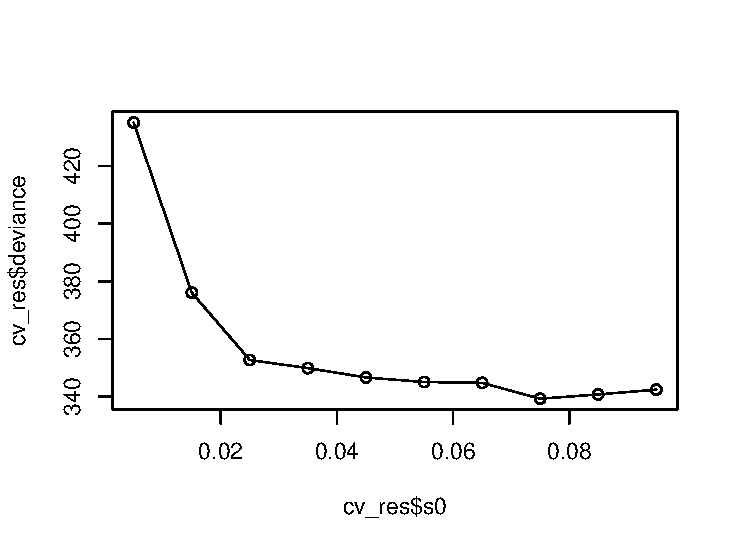
\includegraphics{BHAM_software_files/figure-latex/unnamed-chunk-9-1} \end{center}

\end{CodeChunk}

With the cross-validation results, we can choose from all the candidate
values of \(s_0\) and select the one with the best performance using the
preferred metrics. For example, we can use the \(s_0\) value that gives
the minimum cross-validated deviance, and re-fit the model. Hence, this
would be the optimal model.

\begin{CodeChunk}
\begin{CodeInput}
R> s0_min <- cv_res$s0[which.min(cv_res$deviance)]
R> bham_final <- bamlasso(x = train_smooth_data, y = dat$y,
+                        family = "binomial",
+                        group = make_group(names(train_smooth_data)),
+                        ss = c(s0_min, 0.5))
\end{CodeInput}
\end{CodeChunk}

To note, it is a convention to use some predictive metrics to select the
best performed model among all the candidate values, for both predictive
purpose and variable selection purpose. However, previous literature
shows that when using predictive metrics to select model for variable
selection purpose, the variable selection performance may not be
optimal.

\subsection{Varible Selection and Curve Intropolation}

In the proposed R package, we also provide some utility functions to
provide more insights for the additive function inferences.

\subsubsection{Variable Selecrtion}

We provide a function to summarize the variable selection of the
produced model, namely \texttt{bamlasso\_var\_selection}. The input of
the function is a fitted BHAM model, and the output of the function is a
list of two components, \texttt{parametric} and \texttt{non-parametric}.
The \texttt{parametrc} component is a vector contains the selected
variables that were fitted in the model in its parameteric form,
i.e.~not specified via additive functions. The \texttt{non-parametric}
component contains a dataframe with 3 columns, \texttt{Variable},
\texttt{Linear}, \texttt{Nonlinear}. While \texttt{Variable} column
includes the variable names of selected aadditive functions,
\texttt{Linear} and \texttt{Nonlinear} columns are logical vectors
indicating if the linear and nonlinear components of the additive
function are included in the model respectively.

\begin{CodeChunk}
\begin{CodeInput}
R> bamlasso_vs_part <- bamlasso_var_selection(bham_final)
\end{CodeInput}
\end{CodeChunk}

Here, we shows the variable selection result from previously tuned
model. Since, the model didn't include any variables in their parametric
form. Hence, the \texttt{parametric} is an empty vector. Meanwhile, the
\texttt{nonparametric} data frame contains the bi-level selection
result.

\begin{CodeChunk}
\begin{CodeInput}
R> bamlasso_vs_part
\end{CodeInput}
\begin{CodeOutput}
$Parametric
character(0)

$`Non-parametric`
  Variable Linear Nonlinear
1       x1  FALSE      TRUE
2       x2  FALSE      TRUE
3       x3   TRUE     FALSE
4       x4  FALSE      TRUE
5       x5  FALSE      TRUE
6       x7  FALSE      TRUE
7       x9  FALSE      TRUE
8      x10  FALSE      TRUE
\end{CodeOutput}
\end{CodeChunk}

\subsubsection{Curve Plotting}

We also provide a utility function \texttt{plot\_smooth\_term} to plot
the estimated functions. The function takes in the fitted model, the
variable name, the previously constructed smooth objective to construct
the design matrix, minimum and maximum of the range of the predictors.
The function outputs a \texttt{ggplot} object to show the estimated
curve.

\begin{CodeChunk}
\begin{CodeInput}
R> plot_smooth_term(bham_final, "x1", train_smooth,
+                      min = min(dat[, "x1"]),
+                      max = max(dat[, "x1"]))
\end{CodeInput}
\begin{CodeOutput}
`geom_smooth()` using method = 'loess' and formula 'y ~ x'
\end{CodeOutput}


\begin{center}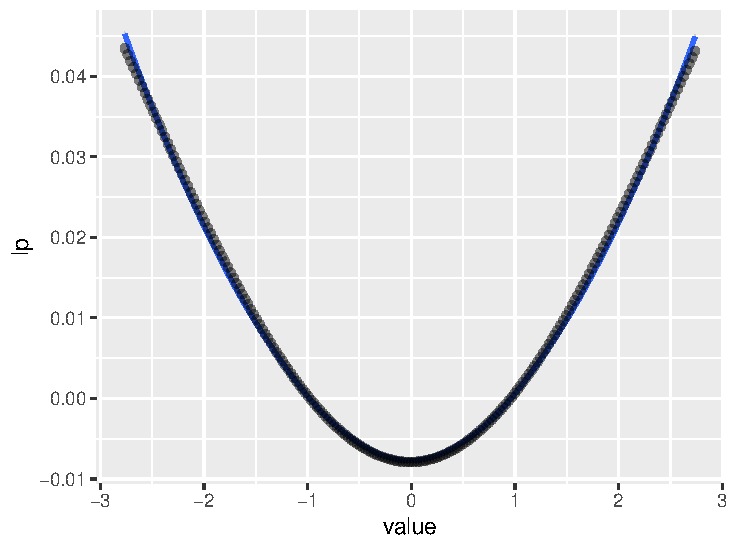
\includegraphics{BHAM_software_files/figure-latex/unnamed-chunk-13-1} \end{center}

\end{CodeChunk}

\subsection{Prediction}

To predict new datasets, we need to go through a two-step procedure as
previously building the model. First of all, we need to translate the
new dataset to their matrix form using the function
\texttt{make\_predict\_dat}. This step is necessary because of the
reparameterization of the design matrix. The function
\texttt{make\_predict\_dat} is based on the function \texttt{PredictMat}
from \texttt{mgcv}. The function asks for an additional input argument
besides the new dataset, i.e.~the Smooth object when constructing the
design matrix for the training data. The output of the function is the
new dataset design matrix with conformable dimension and variable name.
We show the first six columns of the first five observations in the
following example.

\begin{CodeChunk}
\begin{CodeInput}
R> train_smooth <- train_sm_dat$Smooth
R> test_sm_dat <- make_predict_dat(train_sm_dat$Smooth, dat = test_dat)
\end{CodeInput}
\end{CodeChunk}

\begin{CodeChunk}
\begin{CodeOutput}
     x1.pen1     x1.pen2    x1.pen3     x1.pen4    x1.pen5   x1.null1
1  0.2105822 -0.51339049 -0.7087016  1.48599984 -1.6282845 -0.6187856
2  0.1401345 -0.04244866  0.4101826 -2.49600416 -0.5234851  1.2762868
3 -0.1157559 -0.28695472  0.3280699  0.08111065  9.0232660  3.6778234
4 -0.1551403 -0.57575563  1.1032603 -2.71644734  1.1193043  1.8444025
5  0.1841429 -0.50899800 -0.7593021  1.41065378 -1.6744694 -0.5829544
\end{CodeOutput}
\end{CodeChunk}

With the new dataset in the conformable design matrix format, we can
easily produce the prediction using the function \texttt{predict}. Under
the hood, we use \texttt{predict.glmnet} to produce the prediction, and
hence, it is robust. For the GLM, we can produce the linear predictors
using \texttt{type\ =\ "link"} and the fitted probability/mean using
\texttt{type\ =\ "response"}.

\begin{CodeChunk}
\begin{CodeInput}
R> bham_final$offset = 0
R> pred_res <- predict(bham_final, newx = as.matrix(test_sm_dat),
+                     newoffset = 0, type = "link")
\end{CodeInput}
\end{CodeChunk}

To note, we suggest to use \texttt{BhGLM::measure.bh} to provide a quick
prediction performance of the new dataset.

\begin{CodeChunk}
\begin{CodeInput}
R> if(!require("devtools")) install.packages("devtools")
R> if(!require("BhGLM")) devtools::install_github("nyiuab/BhGLM")
R> 
R> BhGLM::measure.bh(bham_final, as.matrix(test_sm_dat), test_dat$y)
\end{CodeInput}
\end{CodeChunk}

\section{Discussion}

In this article, we introduce the R package \texttt{BHAM} to fit
Bayesian Hierarchical additive models with two-part spike-and-slab LASSO
prior for high-dimensional data analysis. The R package can be widely
used to analyze large-scale molecular and clinical data with the
flexibility to model both linear and nonlinear signals, and hence
provide improved prediction accuracy. Meanwhile, compared to the more
complicated machine learning method, the additive models can provide
more interpretable inference of the underlying signals. In addition, the
two-part spike-and-slab LASSO prior for smooth function and the EM-CD
algorithm provides a natural solution to the bi-level selection problem,
without further requirement of thresholding or hypothesis testing.
Fitting a high-dimensional Bayesian model is normally computationally
intensive. We provide an economic solution by integrate coordinate
descent algorithm with the EM procedure. The implementation of the
algorithm leverage some commonly used modeling interface form the
standard R packages and hence granting robustness.

To help the users to familiarize the utilities of \texttt{BHAM}, we
provide a analysis pipeline in this manuscript. We demonstrate the
construction of the design matrix, model fitting and tuning, signal
selection and visualization, and prediction via the analysis of a
simulated data set. Due to the space constraint, we can't showcase all
the functionality offered by \texttt{BHAM} for example fitting a Cox
proportional hazard model, time-varying effect model, or fitting the
model with the EM-Newton or EM-IWLS algorithms. We recommand the user to
visit an interactive website for more details via
\url{https://boyiguo1.github.io/BHAM/}.

Optimal goal is to provide interface for optimal customizability.

\clearpage

\bibliography{references.bib}



\end{document}
